% textidote: ignore begin
\section{User Interface Design}\label{sec:user-interface-design}
% textidote: ignore end

When designing the user interface, the group used an iterative approach~\cite{iterative-design}.
This means that every iteration of the design was tested and evaluated by the group members or by other groups.
The group members would then discuss the design and decide on changes to be made.
Section~\ref{subsec:brainstorming} will introduce the initial brainstorming process, and then, 
Section~\ref{subsec:navigation-map} will introduce the navigation map.
Section~\ref{subsec:lo-fi-prototyping}, Section~\ref{subsec:hi-fi-prototyping} and Section~\ref{subsec:final-design}
will introduce the process of creating the user interface itself and how the design went from early sketches to a
finished program.
Finally, Section~\ref{subsec:heuristics} will look into the heuristics used to evaluate the final design.

\subsection{Brainstorming}\label{subsec:brainstorming}

Before starting on the actual design, the group agreed to have one brainstorming session, where everyone would share
their ideas on how the user interface should look.
Each group member presented their ideas either verbally or through sketches.
From those ideas, the group agreed on a number of key features that the user interface should have.
Everyone agreed that the final interface should be in the form of a dashboard, and that the data from
the~\acrshort{epos} should be visualized in the form of a chart.

\begin{figure}[H]
    \centering
    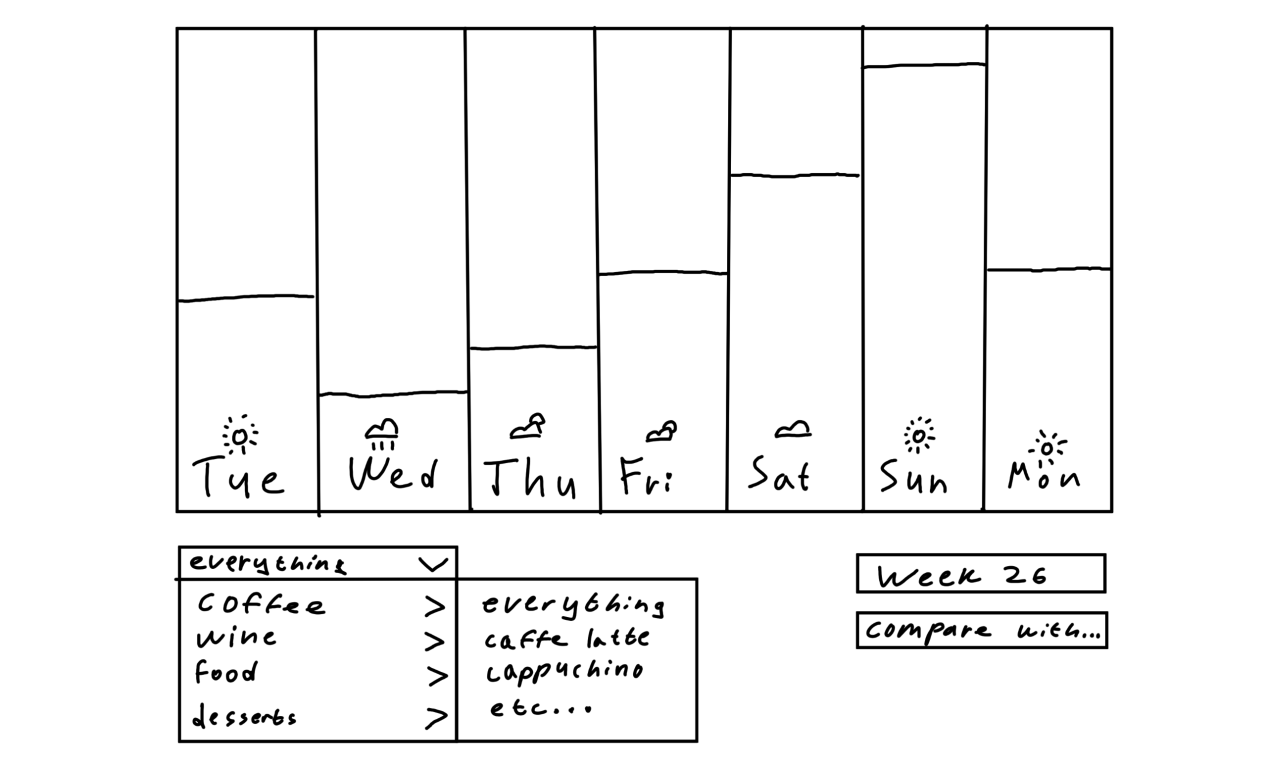
\includegraphics[width=\textwidth]{design-early.png}
    \caption{An example of an early chart.
    }\label{fig:design-early}
\end{figure}

The team decided on prioritizing two charts: A bar chart and a heatmap.
The functionality and choice rationale for these charts are explained in
Section~\ref{subsubsec:relevant-visualization-types}.
Figure~\ref{fig:design-early} shows an early prototype of a bar chart.
The designs and ideas were shared with the client, who approved of the direction the group was taking.

\subsection{Navigation map}\label{subsec:navigation-map}

After the brainstorming session, the group started to create a navigation map~\cite{benyon2019}.
This map was made to visualize the flow of the user interface.
It features the different pages and how they are connected.
The navigation map can be seen in Figure~\ref{fig:navigation-map}.
Do note that the navigation map is representative of the final design and not the design of the prototypes.

The first page that the user interacts with is the login page.
From there they are directed to the dashboard, but they also have the choice to switch between the settings page and a
list of all the uploaded data.
The main focus for this project is the dashboard, where the user can see the different charts.
The settings page would allow the users to upload the data from their~\acrshort{epos} and to create categories for the
charts.
The total sales page shows a list of all the data without any visualization.
The user can also see visualization for a specific day from either the dashboard or the total sales page.

\begin{figure}[H]
    \centering
    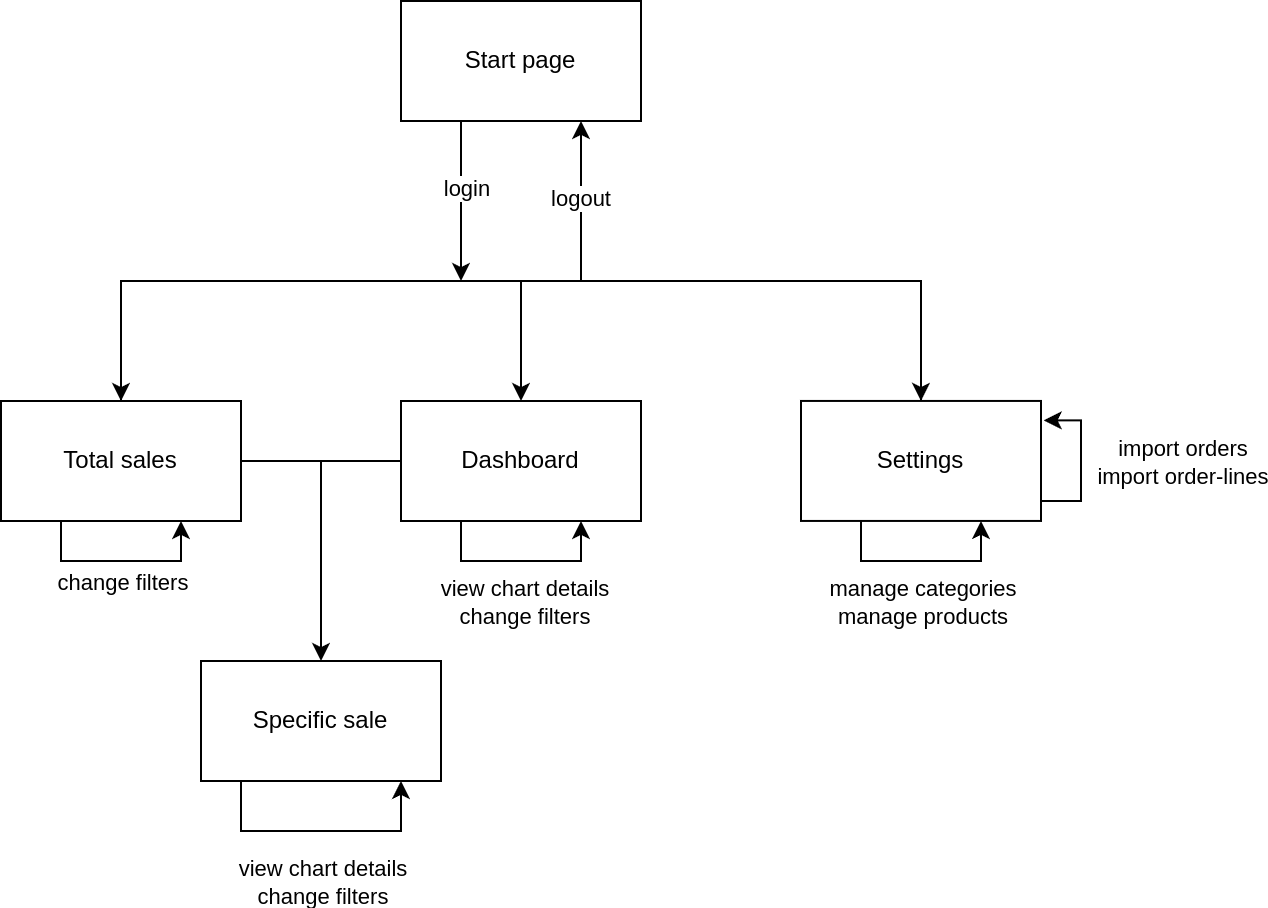
\includegraphics[width=\textwidth]{design-navigation-map.png}
    \caption{Navigation map of the final design.
    }\label{fig:navigation-map}
\end{figure}

\subsection{Lo-Fi Prototyping}\label{subsec:lo-fi-prototyping}

After the early prototyping phase, the group started to create a low-fidelity prototype~\cite{hi-lo-fidelity}.
This was done during a hackathon week, where the group had the opportunity to work on the prototypes together with
other groups.
Therefore, the group got a lot of feedback from other groups, which helped to improve the design.
The specific feedback is discussed in Section~\ref{sec:evaluation}.

This design, which can be seen in Figure~\ref{fig:lofi-prototype}, is made out of pen and paper.
It is made to be modular, which means that different charts and options can be attached or removed.
This encourages interactivity when testing the prototype.
The design focuses on a single chart at a time with an option to filter
the data using the calendar view on the bottom.
The charts can be switched between using the buttons on either side of the chart.
The calendar on the bottom can be clicked on to filter data for a specific time period.
The examples in the figure include:

\begin{itemize}
    \item The login page as seen in Figure~\ref{subfig:lofi-login}.
    This is the page where the user attempts to log in to the application.
    \item The upload page as seen in Figure~\ref{subfig:lofi-upload}.
    This is where the user attempts to upload a CSV file with order data.
    \item The bar chart and heatmap as seen in Figure~\ref{subfig:lofi-bar} and~\ref{subfig:lofi-heatmap} respectively.
    These are both components that show the user some data.
\end{itemize}

\begin{figure}[H]
    \centering
    \begin{subfigure}{.49\textwidth}
        \centering
        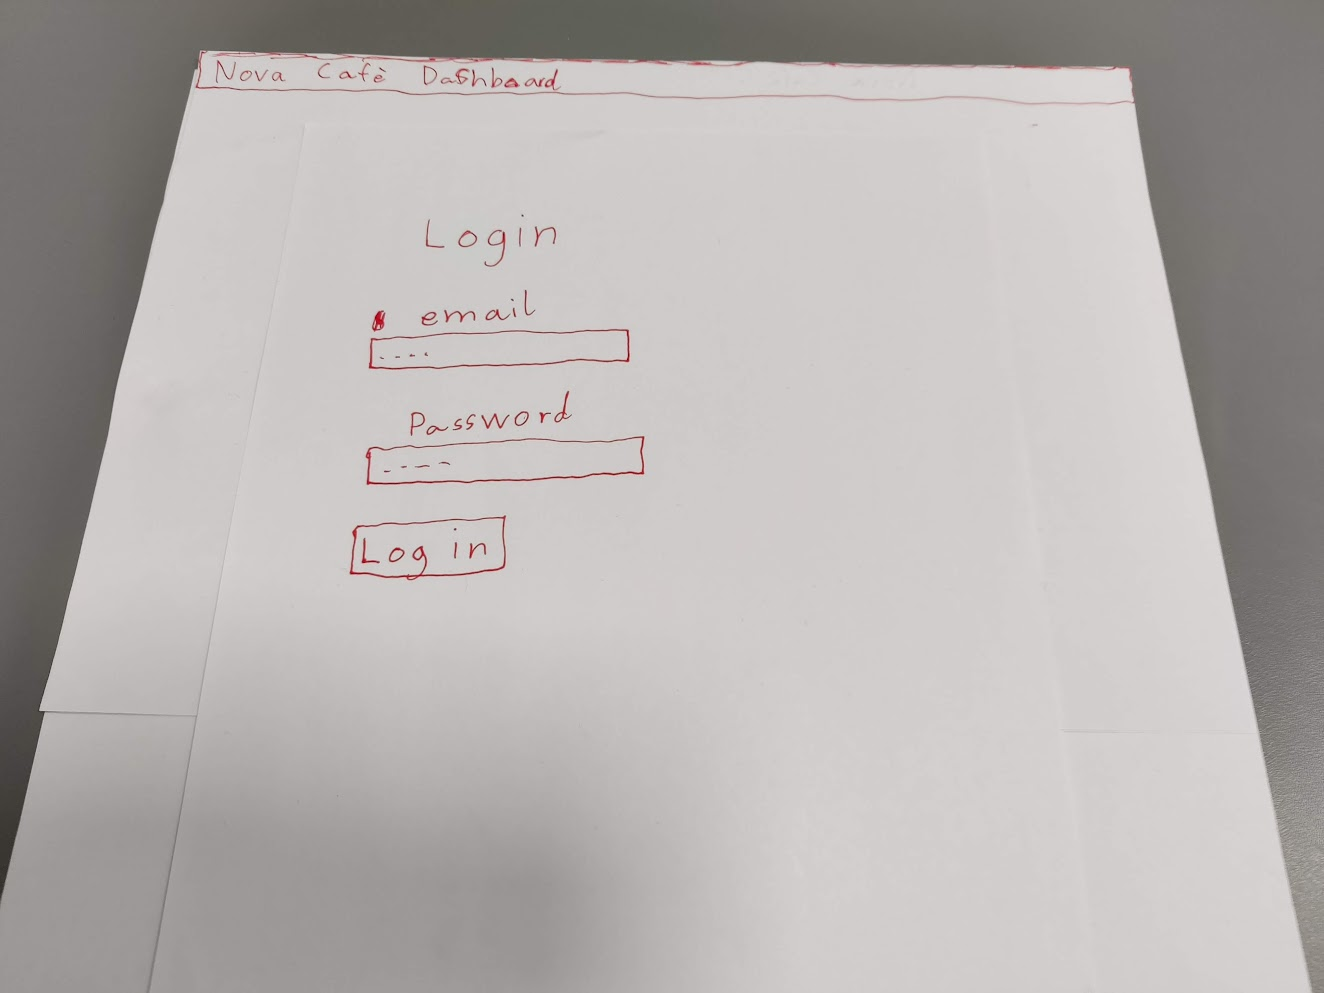
\includegraphics[width=\linewidth]{design-lofi-login}
        \caption{Login page.
        }\label{subfig:lofi-login}
    \end{subfigure}
    \begin{subfigure}{.49\textwidth}
        \centering
        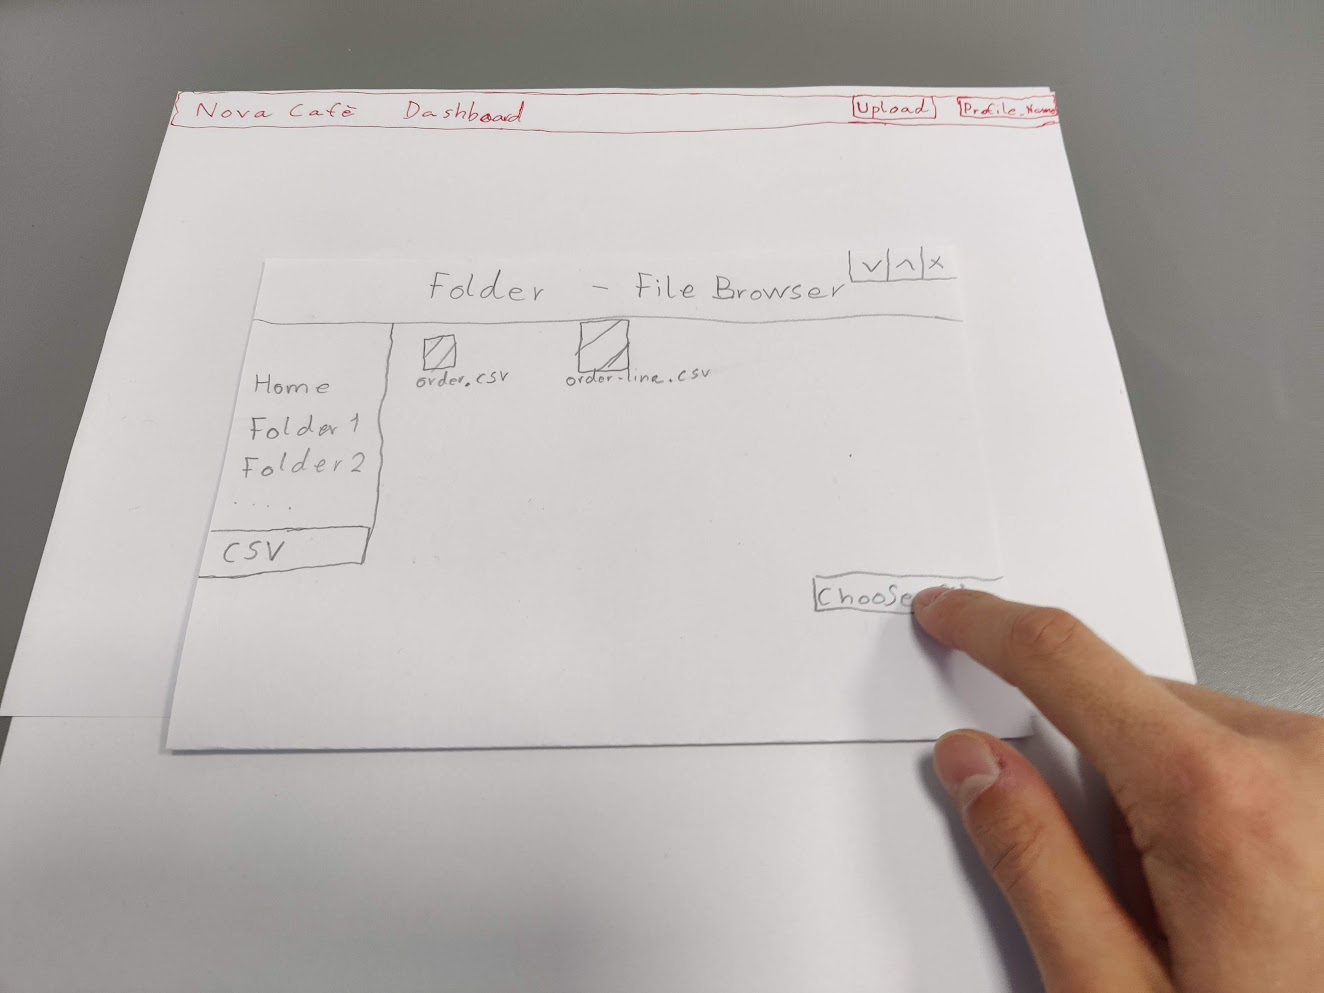
\includegraphics[width=\linewidth]{design-lofi-upload}
        \caption{Upload page.
        }\label{subfig:lofi-upload}
    \end{subfigure}
    \par\medskip
    \begin{subfigure}{.49\textwidth}
        \centering
        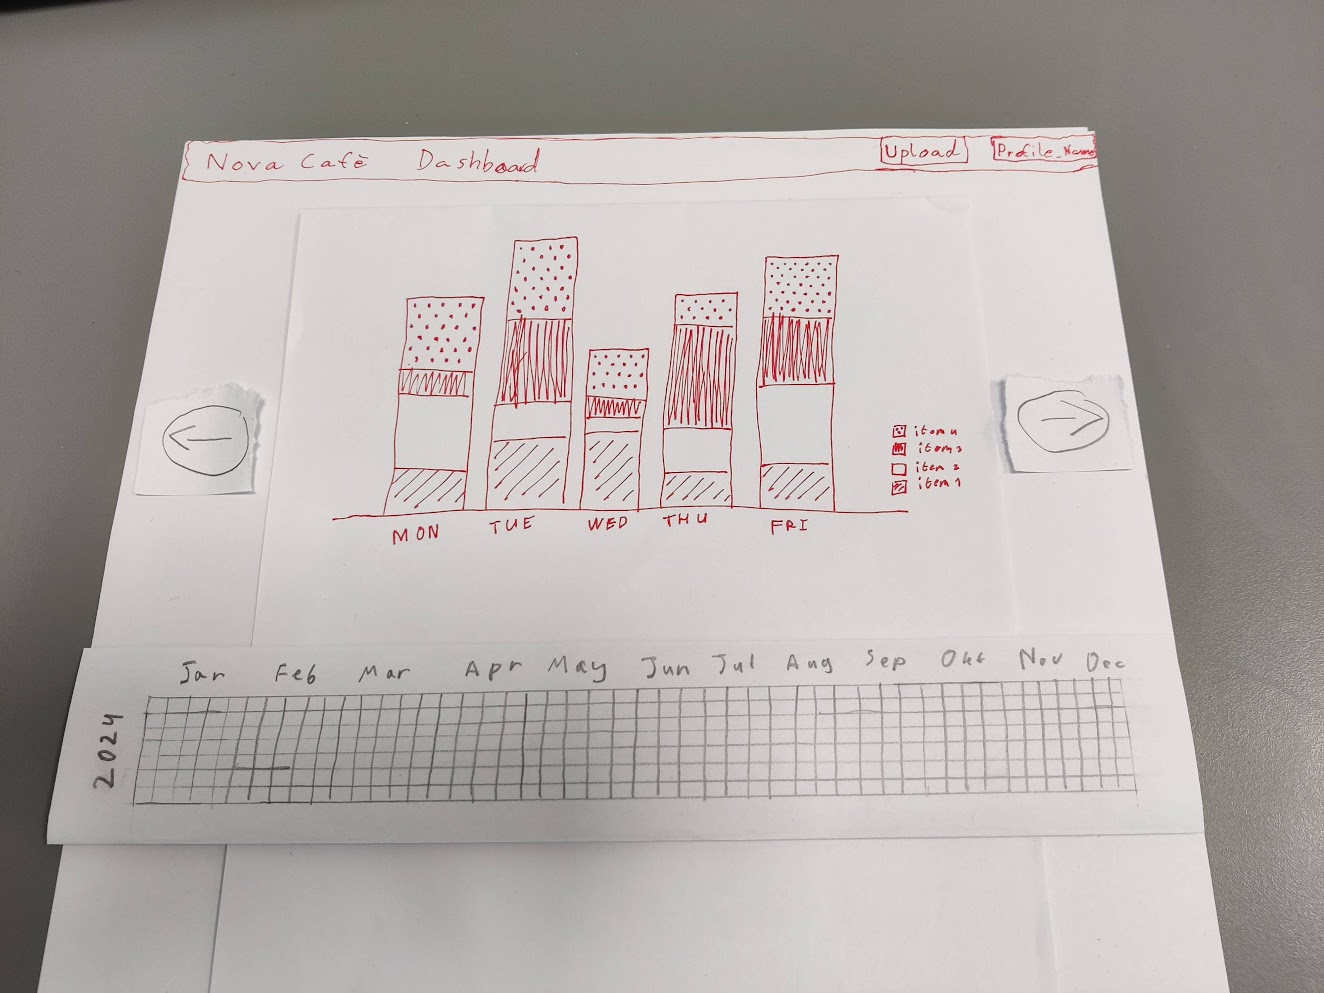
\includegraphics[width=\linewidth]{design-lofi-bar}
        \caption{Bar chart.
        }\label{subfig:lofi-bar}
    \end{subfigure}
    \begin{subfigure}{.49\textwidth}
        \centering
        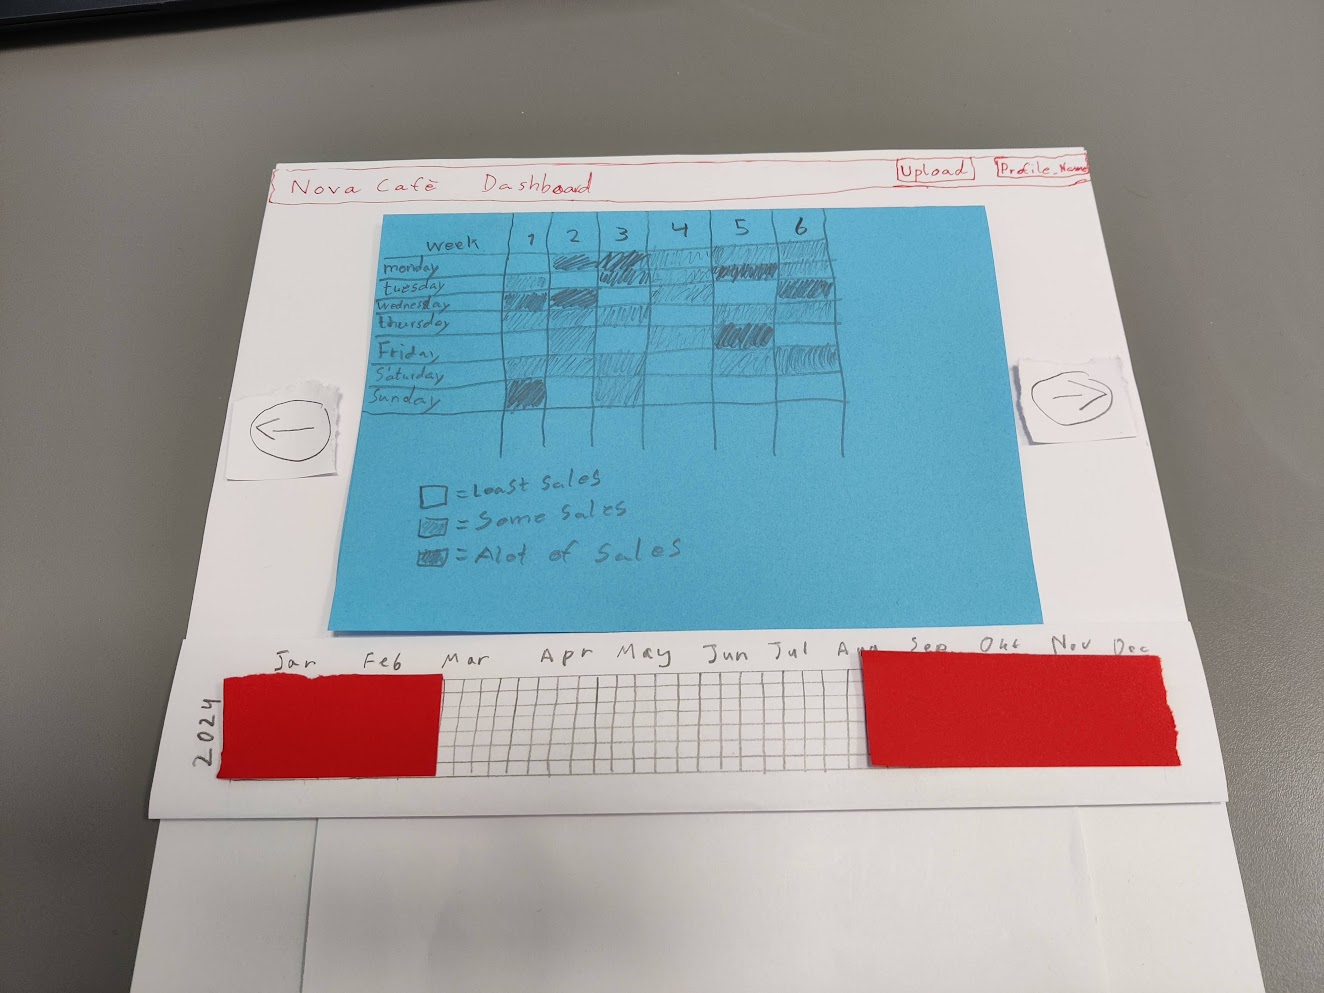
\includegraphics[width=\linewidth]{design-lofi-heatmap}
        \caption{Heatmap.
        }\label{subfig:lofi-heatmap}
    \end{subfigure}
    \caption{Lo-fi prototypes of four components.
    }\label{fig:lofi-prototype}
\end{figure}

\subsection{Hi-fi prototyping}\label{subsec:hi-fi-prototyping}

During the course of the hackathon week, the group also made a high-fidelity prototype~\cite{hi-lo-fidelity}.
This prototype was made within the software solution itself, but without logic behind it and with mock data.
Doing this allowed for an easier transition from the prototype to the final product.
It also represented a more accurate experience of the final product, which made it easier to test and evaluate.

The hi-fi prototype, which can be seen in Figure~\ref{fig:hifi-prototype} is similar to the lo-fi prototype, but with a
more polished look.
The look of the charts is very close to the final design, minus a few minor changes that were made after the group
received feedback for the prototype.
This iteration does not communicate with the back-end, so the data is static.
It is also impossible to filter the data using the calendar view, as this feature would require a database connection.

The group could not implement the feedback they got for the lo-fi prototype, as the hi-fi prototype was made before
the feedback was received.
Instead, the feedback was used to improve the final design.
The examples in the figure include the bar chart and heatmap as seen in Figure~\ref{subfig:hifi-bar}
and~\ref{subfig:hifi-heatmap} respectively.
These are again both components that show the user some data.

\begin{figure}[H]
    \centering
    \begin{subfigure}{.75\textwidth}
        \centering
        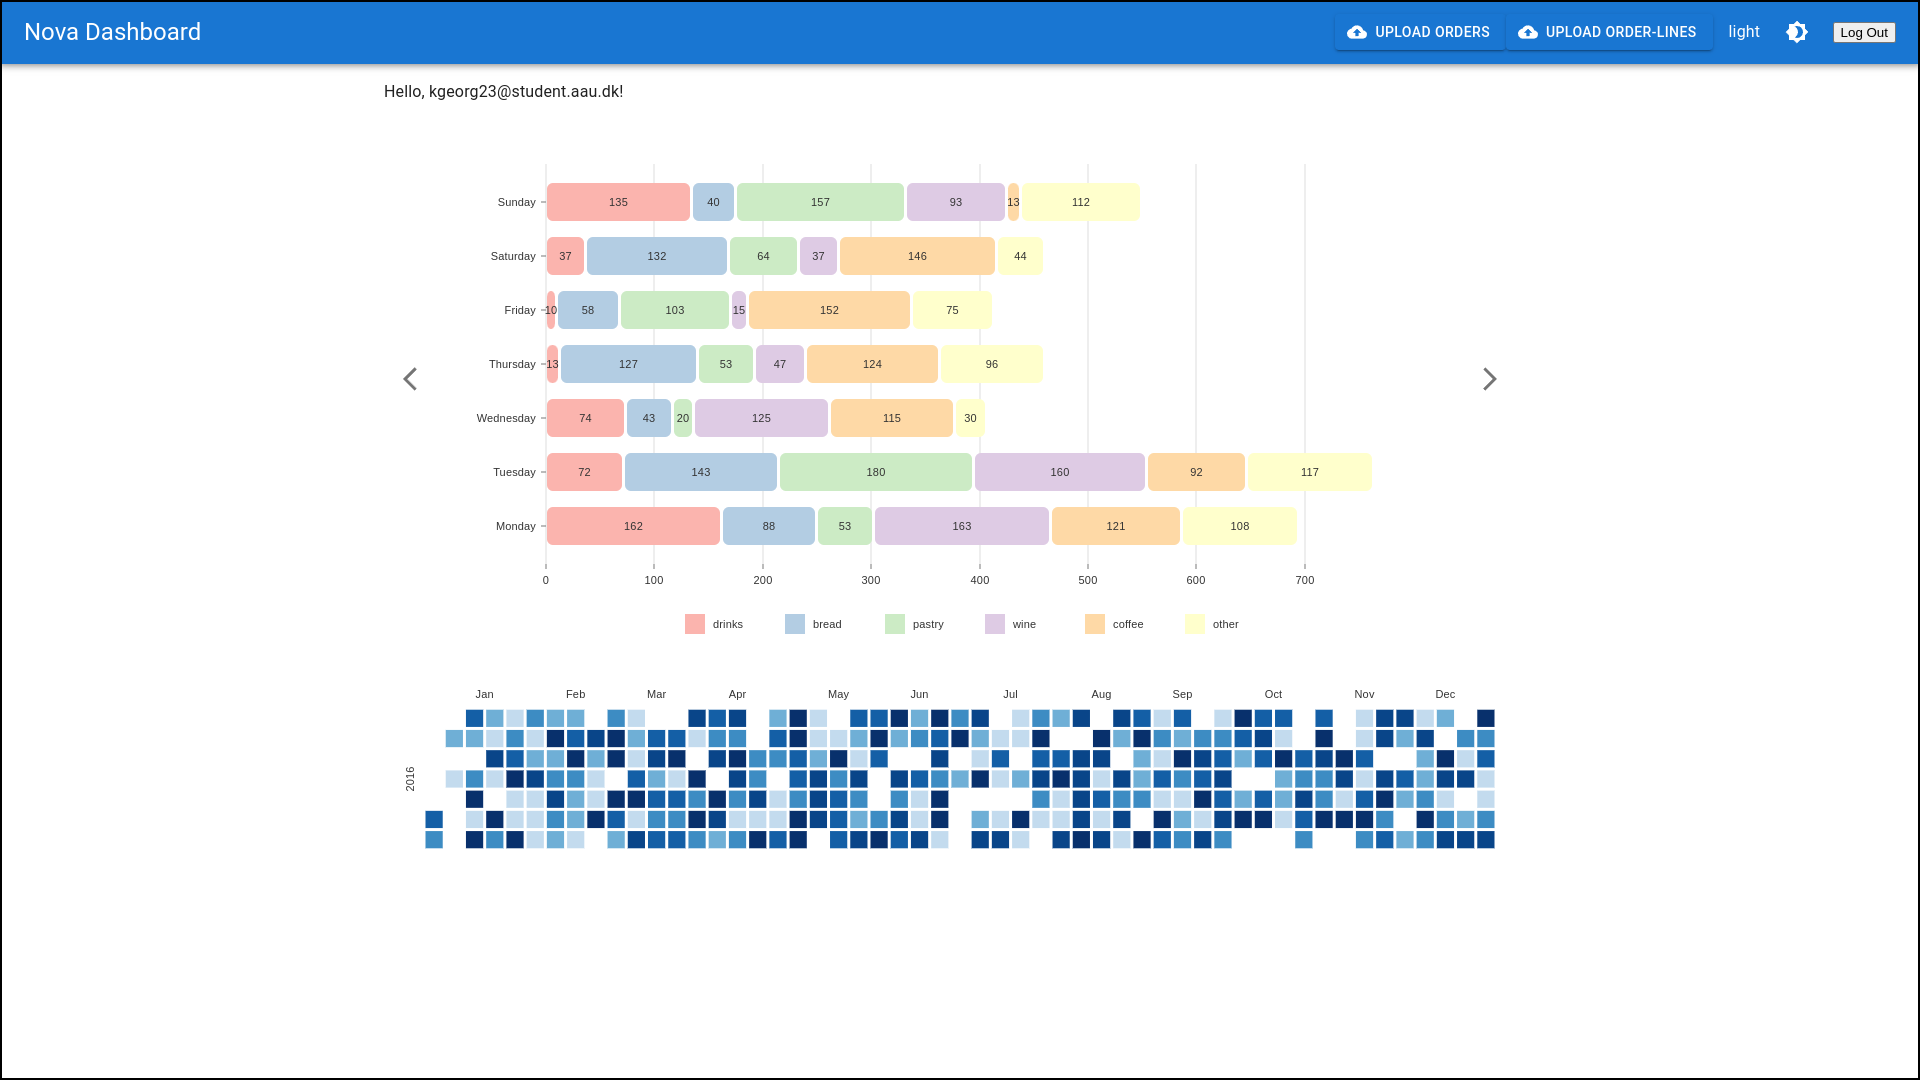
\includegraphics[width=\linewidth]{design-hifi-bar}
        \caption{Bar chart.
        }\label{subfig:hifi-bar}
    \end{subfigure}
    \par\medskip
    \begin{subfigure}{.75\textwidth}
        \centering
        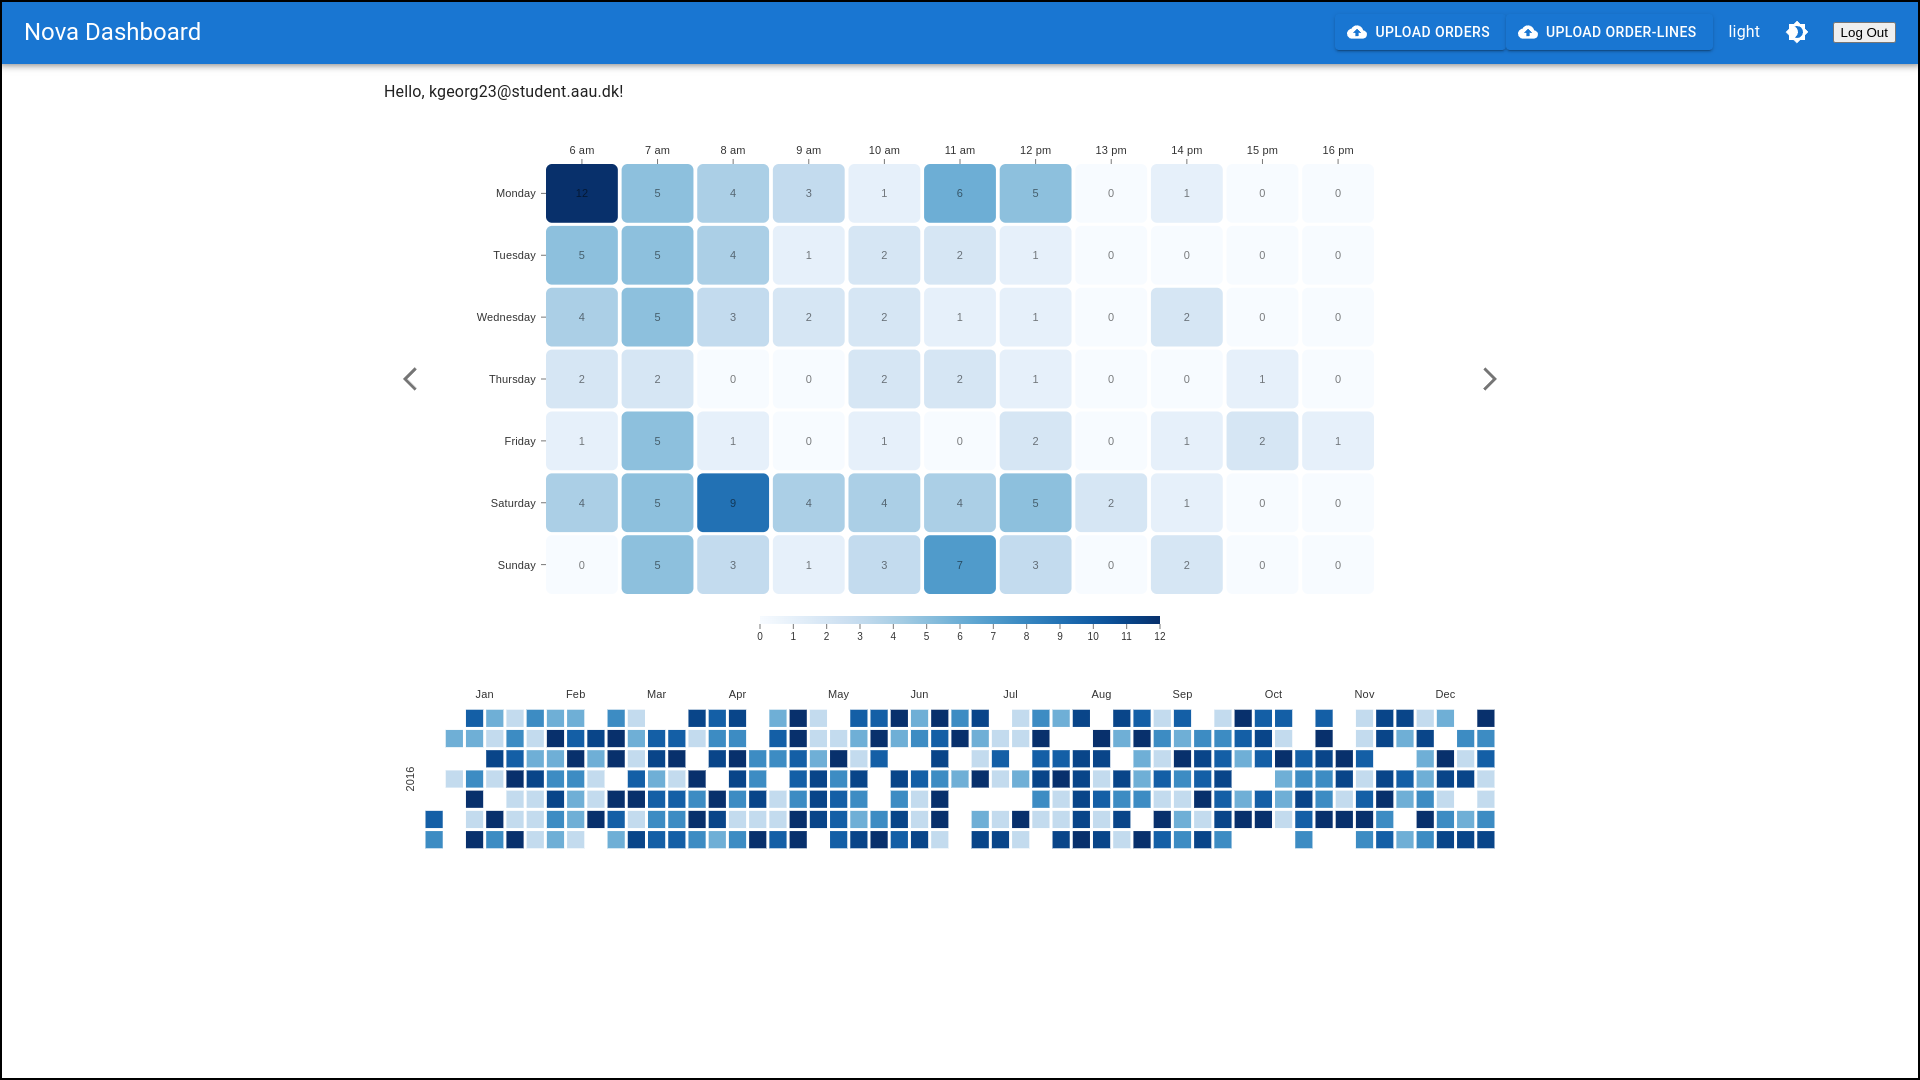
\includegraphics[width=\linewidth]{design-hifi-heatmap}
        \caption{Heatmap.
        }\label{subfig:hifi-heatmap}
    \end{subfigure}
    \caption{Hi-fi prototypes.
    }\label{fig:hifi-prototype}
\end{figure}

\subsection{Final Design}\label{subsec:final-design}

For the final design, the group went back to the hi-fi prototype and made some changes.
The group took into consideration their target audience when designing the user interface.
The interface is minimalistic, and the colors are simple to appeal to the co-workers at the café are mostly young
adults.
For gradient transitions, the group is using shades of blue, with darker shades representing higher values and lighter
shades representing lower values.
Blue was chosen as it contrasts well with its shades, which makes it easy to read the charts.
One requested change for the dashboard was to show more charts at the same time.
This was done by making the charts smaller and adding charts below each other.
These changes can be seen in Figure~\ref{fig:design-final-dash1} and Figure~\ref{fig:design-final-dash2}.

\begin{figure}[H]
    \centering
    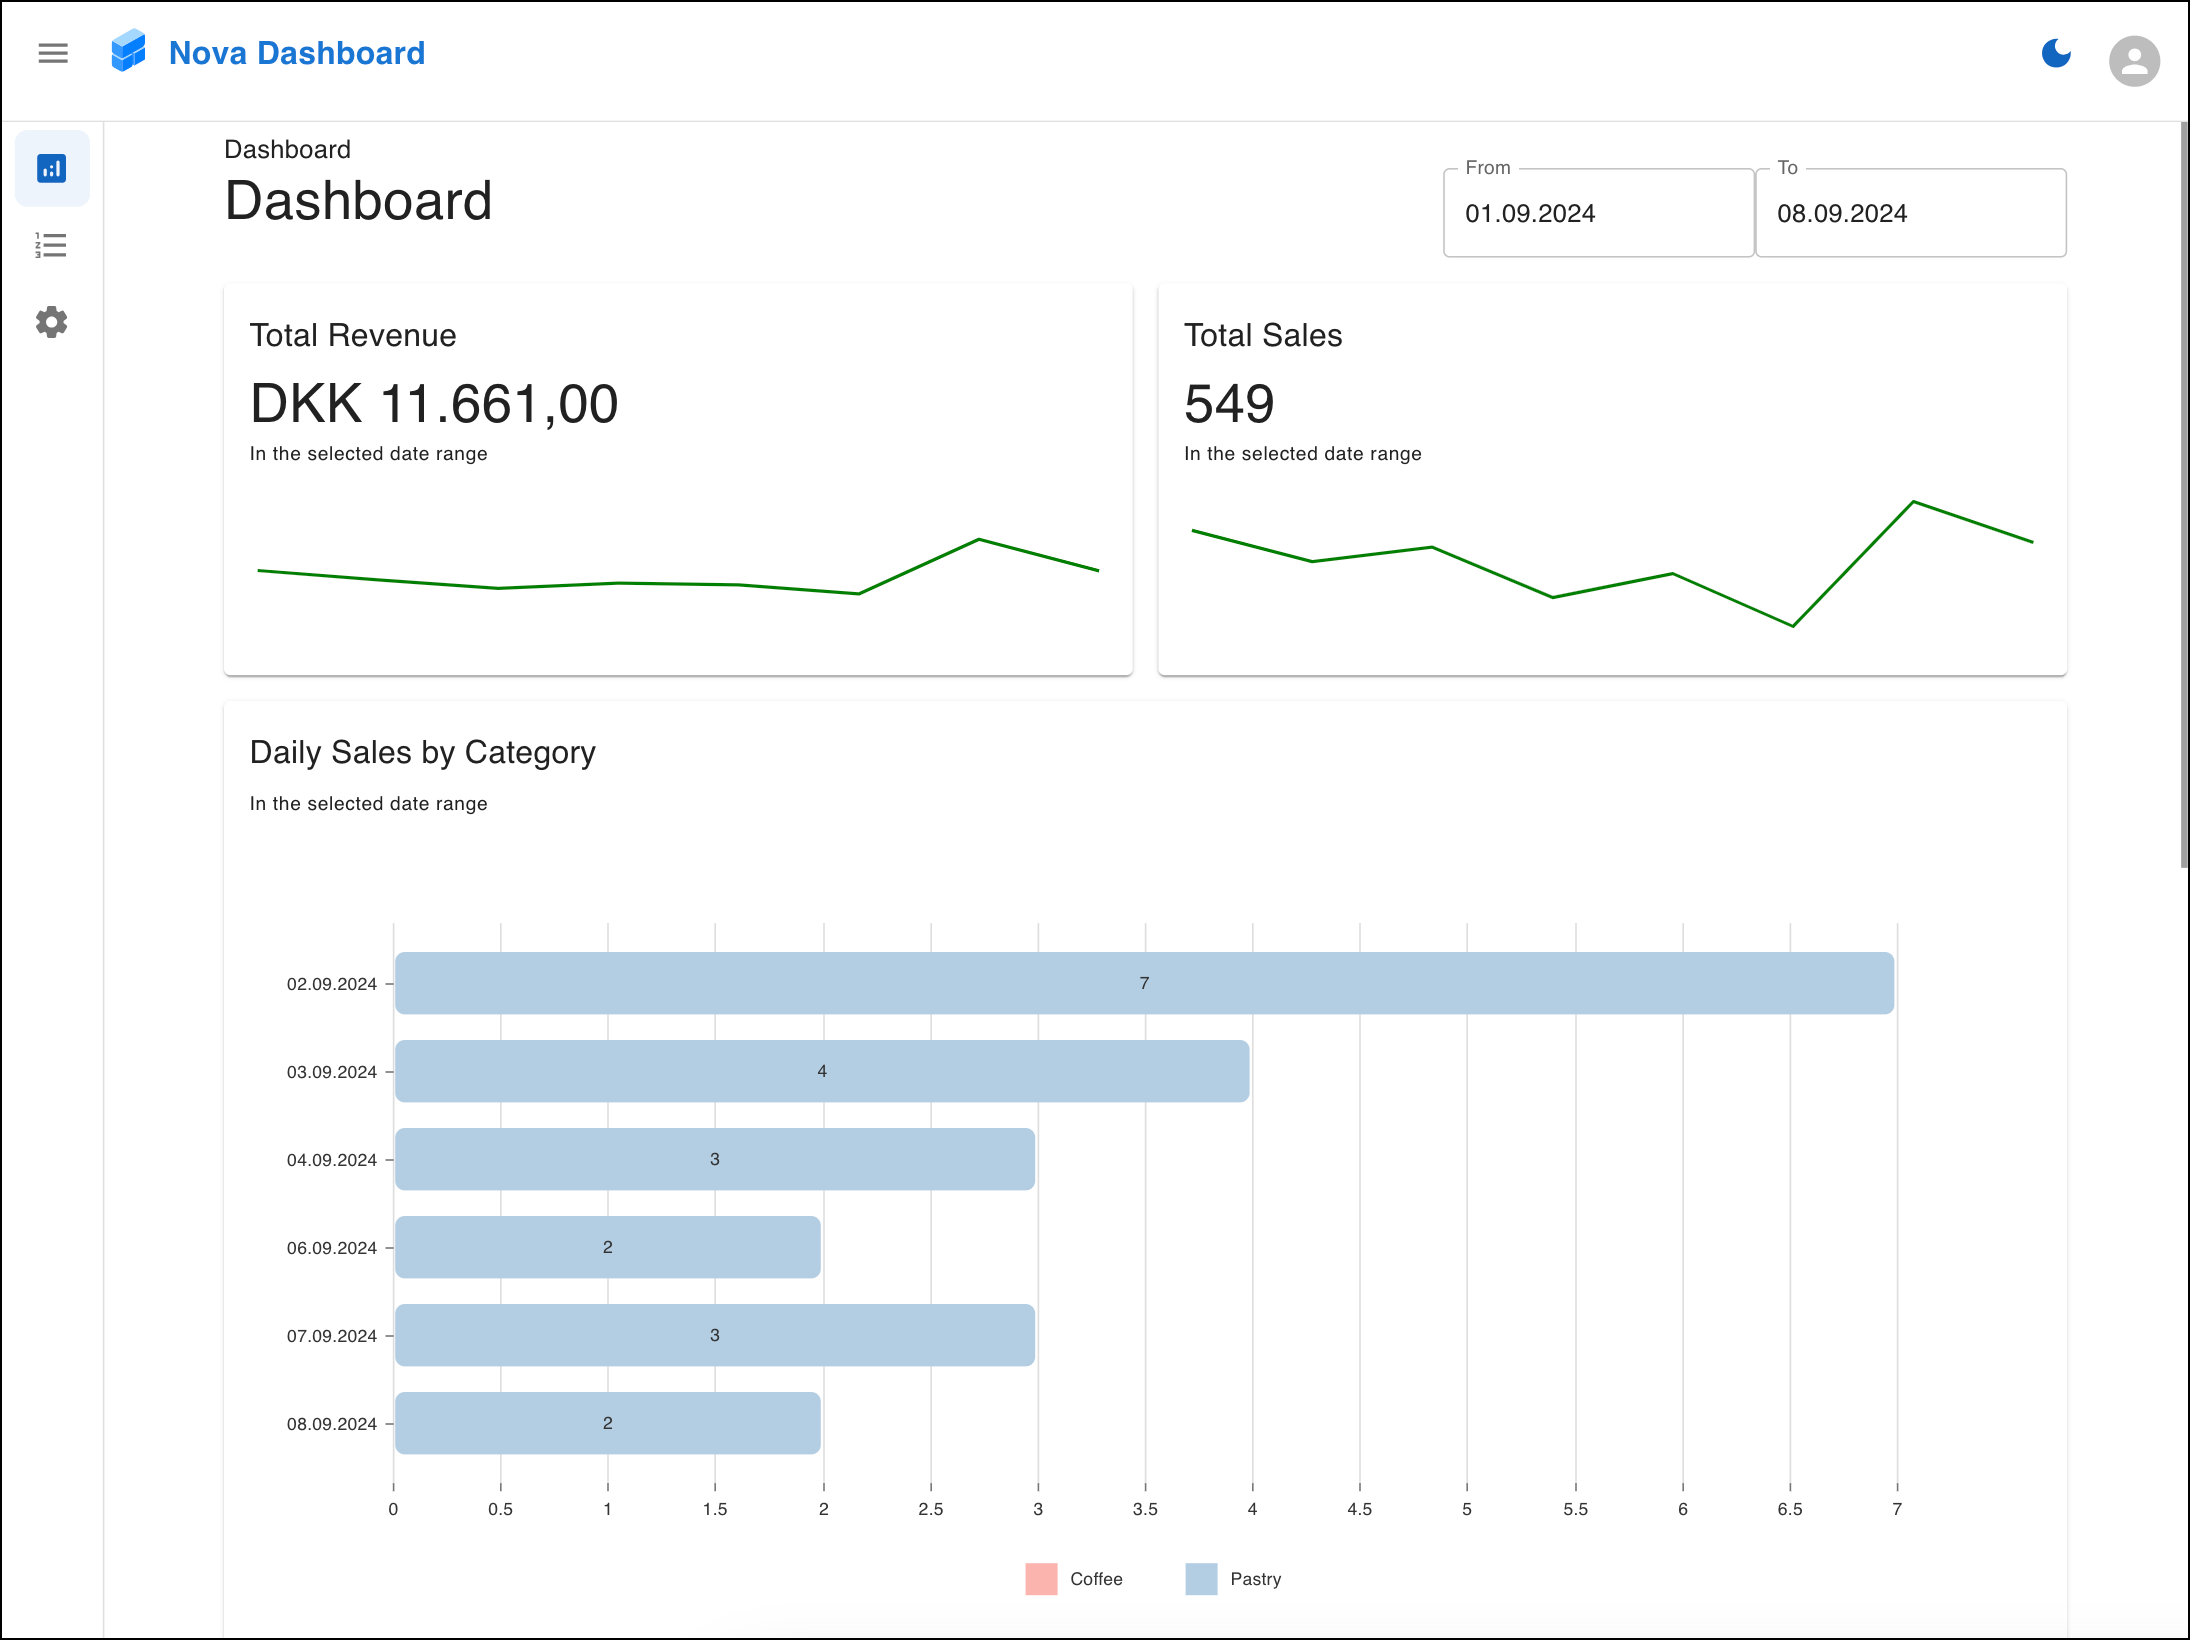
\includegraphics[width=.8\textwidth]{design-final-dash1.png}
    \caption{Final design of the dashboard, upper half.
    }\label{fig:design-final-dash1}
\end{figure}

\begin{figure}[H]
    \centering
    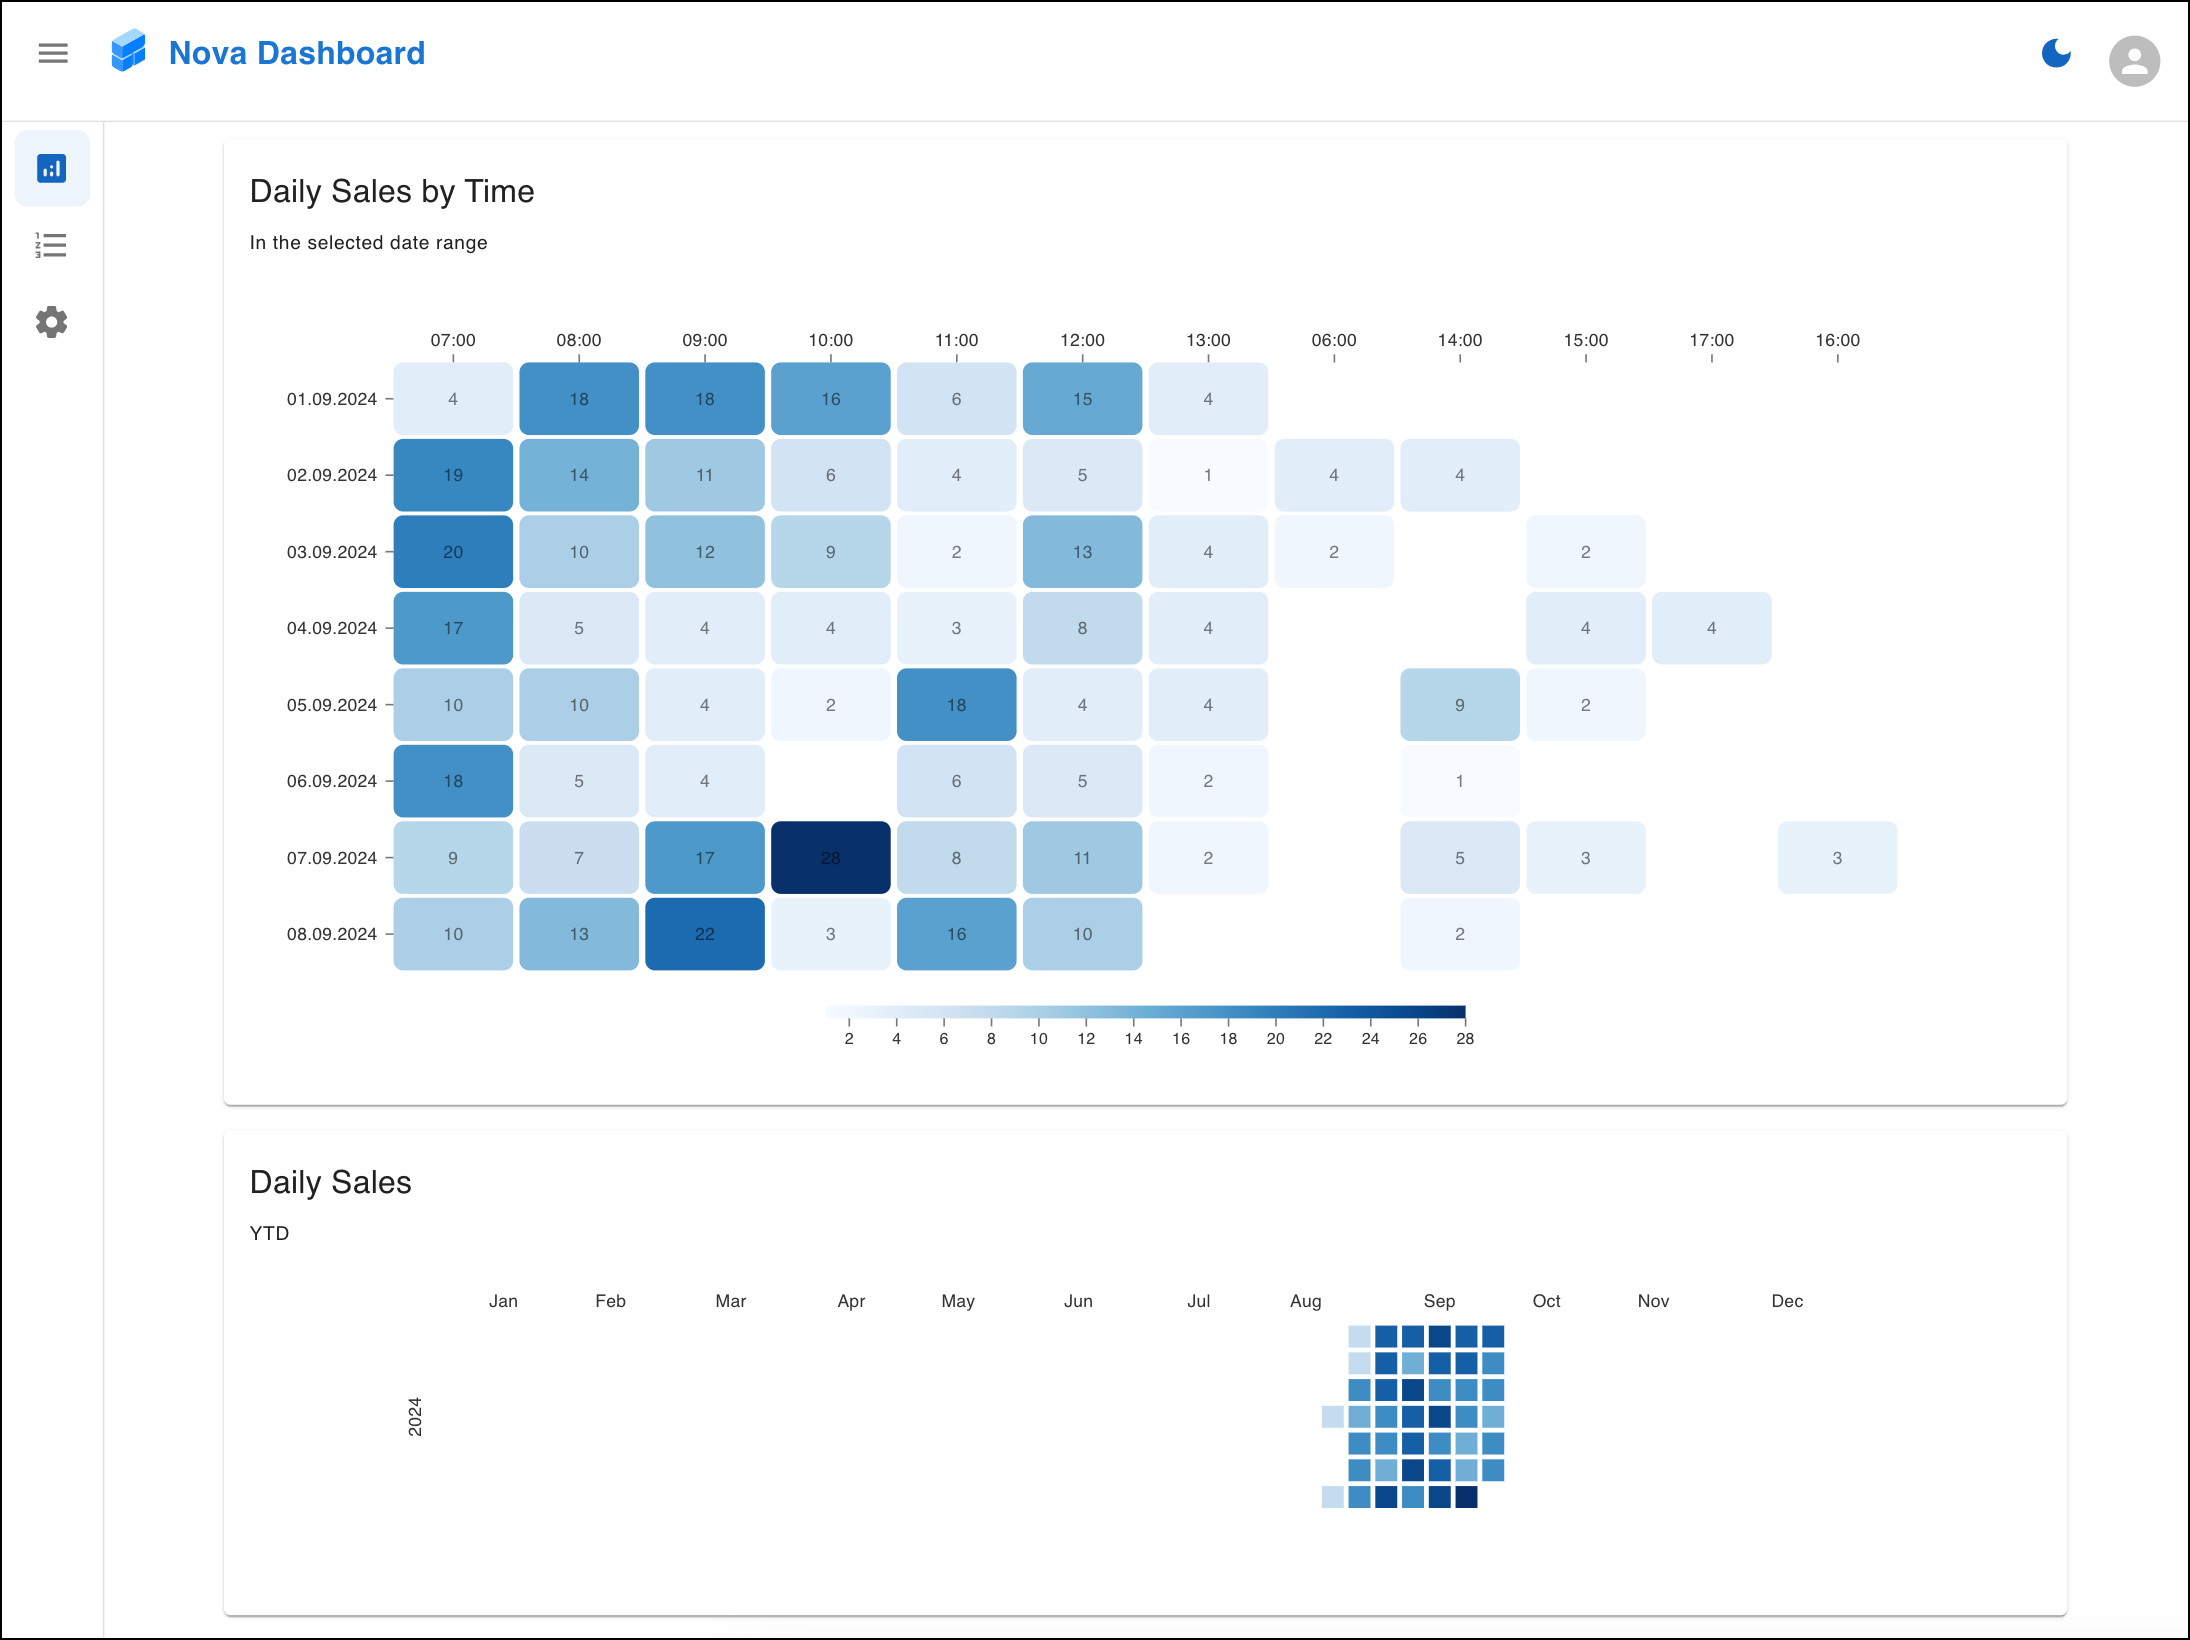
\includegraphics[width=.8\textwidth]{design-final-dash2.png}
    \caption{Final design of the dashboard, lower half.
    }\label{fig:design-final-dash2}
\end{figure}

More pages were added to the final design.
These pages deemed necessary for the application to be fully functional.
A settings page was added, where the upload buttons have been moved to.
This was done to clear up the dashboard and make it less cluttered.
The settings page also allow the user to create and assign categories to items.
The page can be seen in Figure~\ref{fig:design-final-settings} and the act or assigning categories can be seen in
Figure~\ref{fig:design-final-categories}.
Upon successful data upload request, a notification will appear on the bottom left of the screen, as seen in
Figure~\ref{fig:design-final-notification}.

\begin{figure}[H]
    \centering
    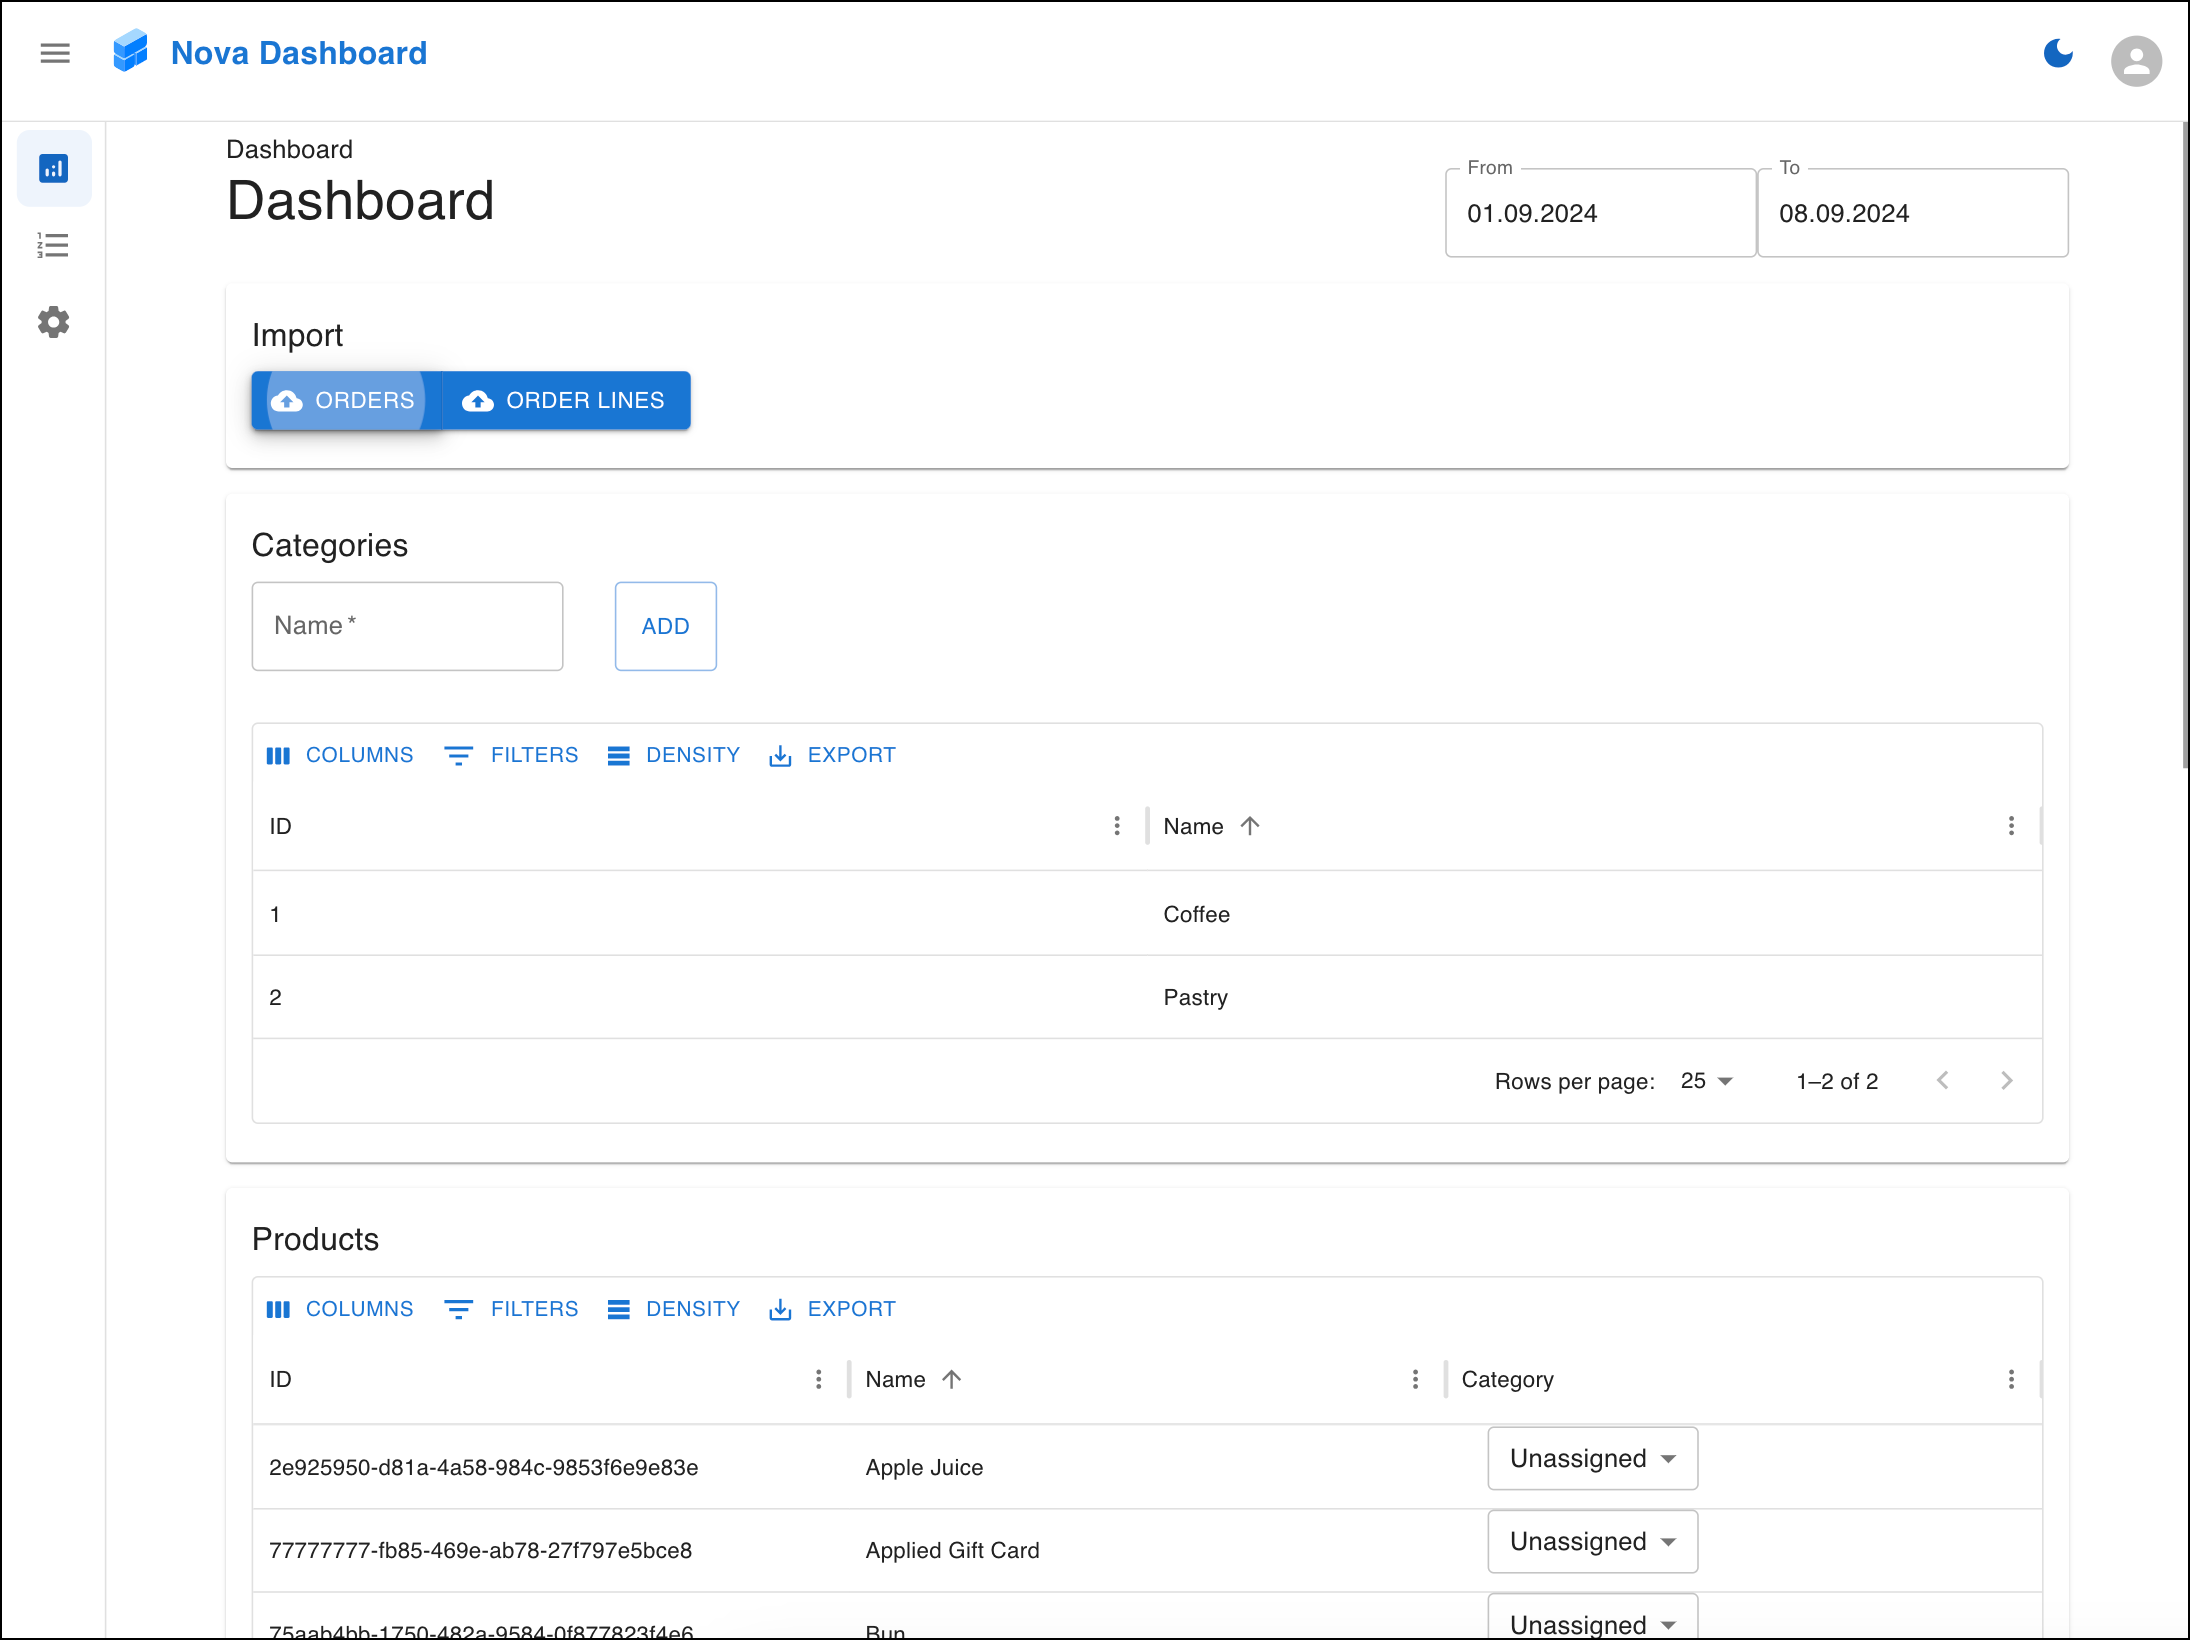
\includegraphics[width=.8\textwidth]{design-final-settings.png}
    \caption{Final design of the settings screen.
    }\label{fig:design-final-settings}
\end{figure}

\begin{figure}[H]
    \centering
    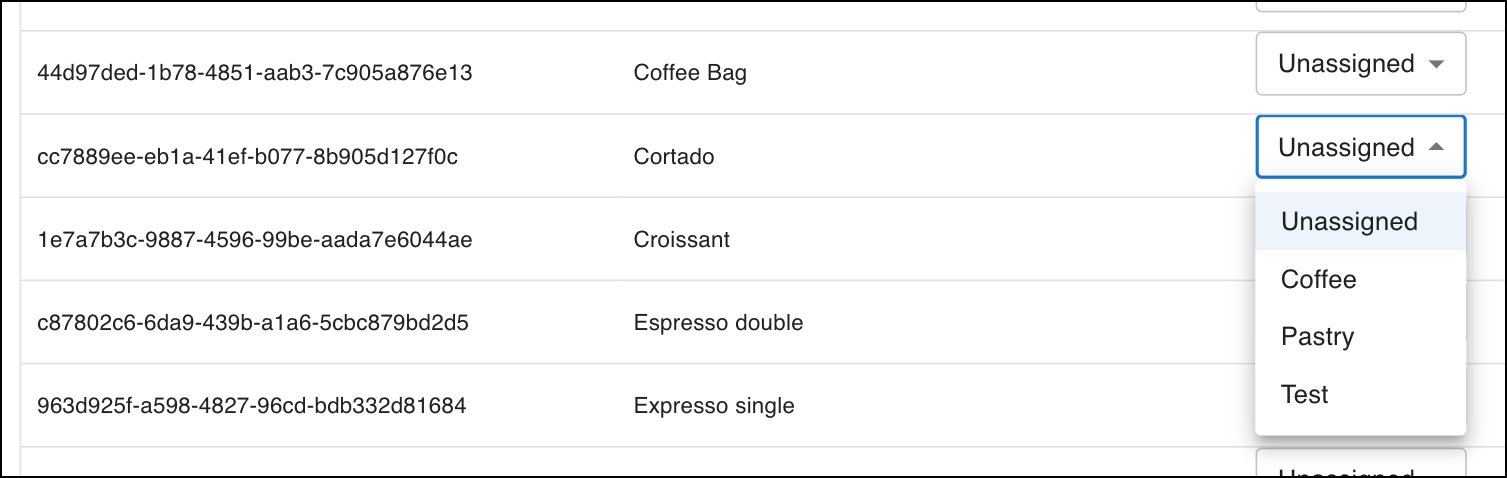
\includegraphics[width=.7\textwidth]{design-final-categories.png}
    \caption{Attaching categories to items.
    }\label{fig:design-final-categories}
\end{figure}

\begin{figure}[H]
    \centering
    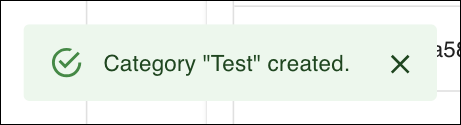
\includegraphics[width=.3\textwidth]{design-final-notification.png}
    \caption{Notification upon successful data upload request.
    }\label{fig:design-final-notification}
\end{figure}

The last page that was added is the sales page.
This page shows a list of all sales that have been made as raw data.
The page can be seen in Figure~\ref{fig:design-final-sales}.

\begin{figure}[H]
    \centering
    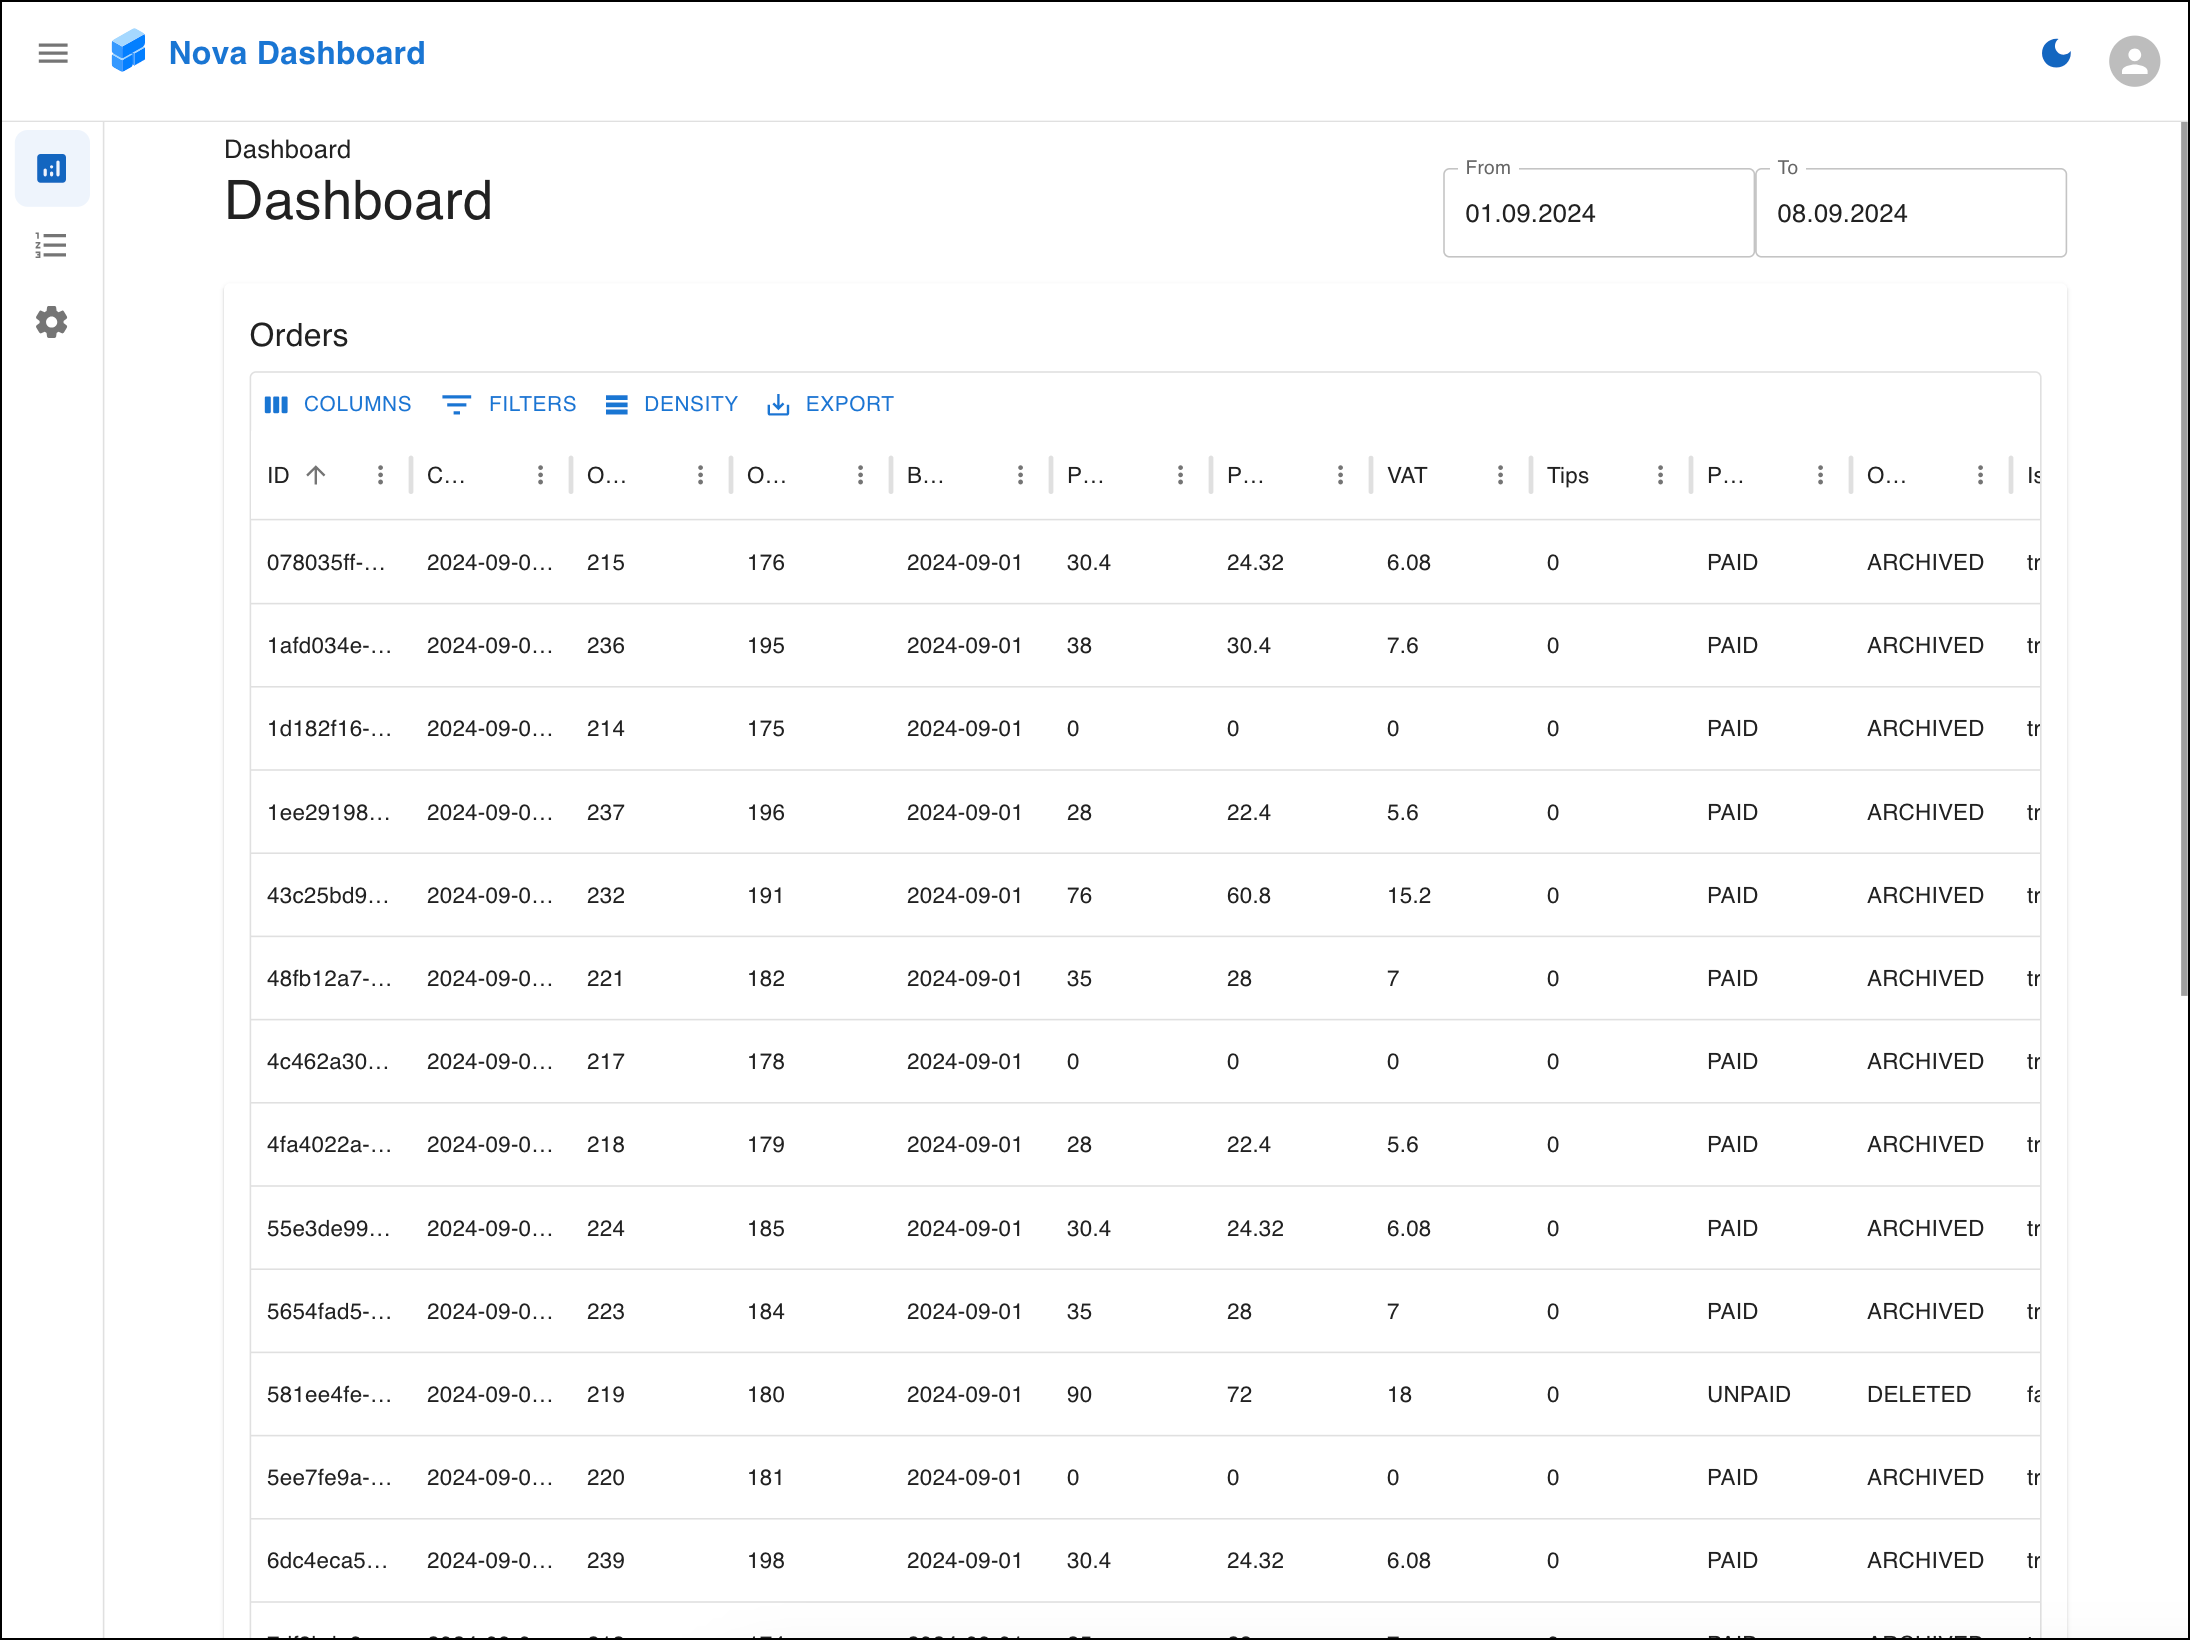
\includegraphics[width=.8\textwidth]{design-final-sales.png}
    \caption{Final design showing the full list of sales.
    }\label{fig:design-final-sales}
\end{figure}

Several functionalities were added to improve the user experience.
Most notably, the group added a functional filter to the dashboard.
There are two buttons on the top right of the dashboard that allows the user to filter the data by entering a specific
date range.
The date picker can be seen in Figure~\ref{fig:design-final-filter}.

\begin{figure}[H]
    \centering
    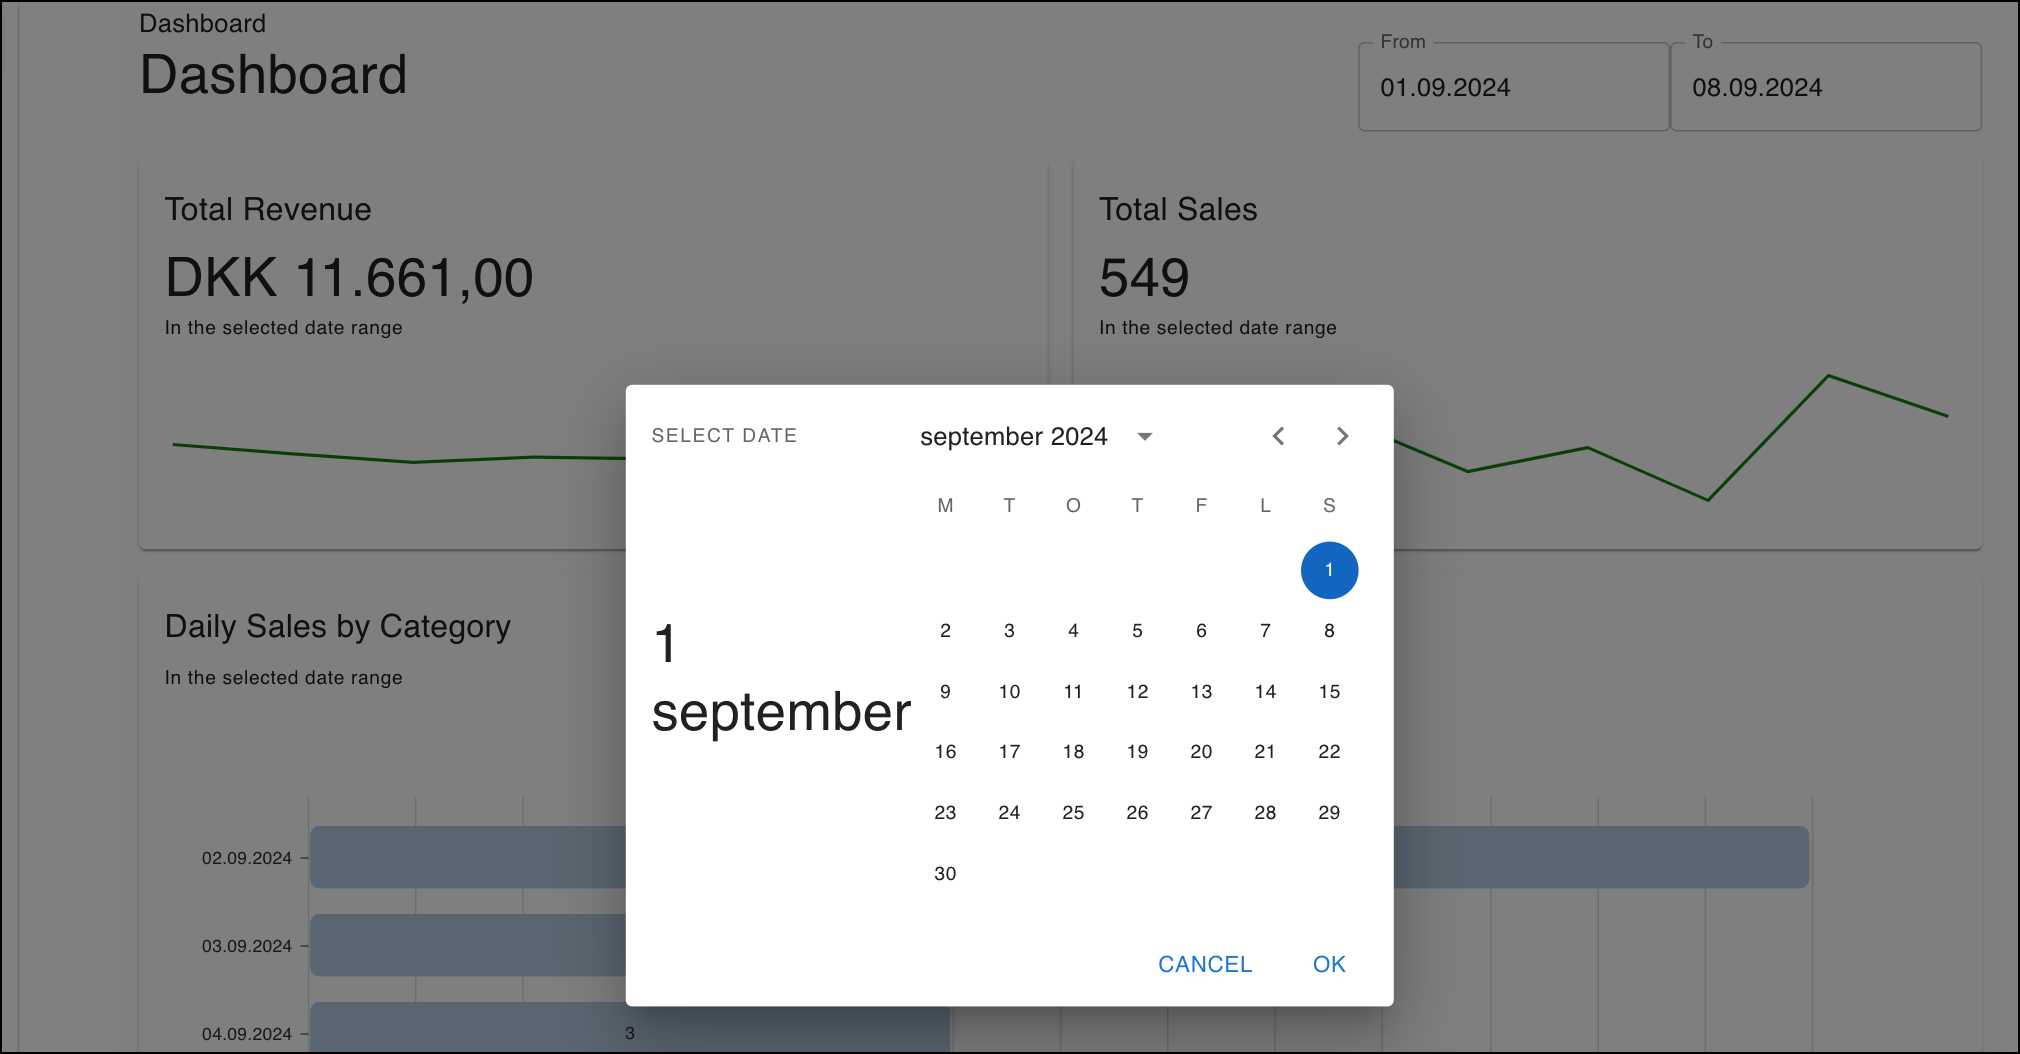
\includegraphics[width=.7\textwidth]{design-final-filter.png}
    \caption{Data filtering using a calendar.
    }\label{fig:design-final-filter}
\end{figure}

Lastly, to improve the usability on a tablet, the navigation bar was moved from the top to the side of the page.
This allows for more vertical space for the charts.
The navigation bar is collapsible, and the user can expand it by clicking the hamburger menu.
This was again done to allow for more space for the charts.
The prior charts show the collapsed navigation bar, and the expanded navigation bar can be seen in
Figure~\ref{fig:design-final-menu}.

\begin{figure}[H]
    \centering
    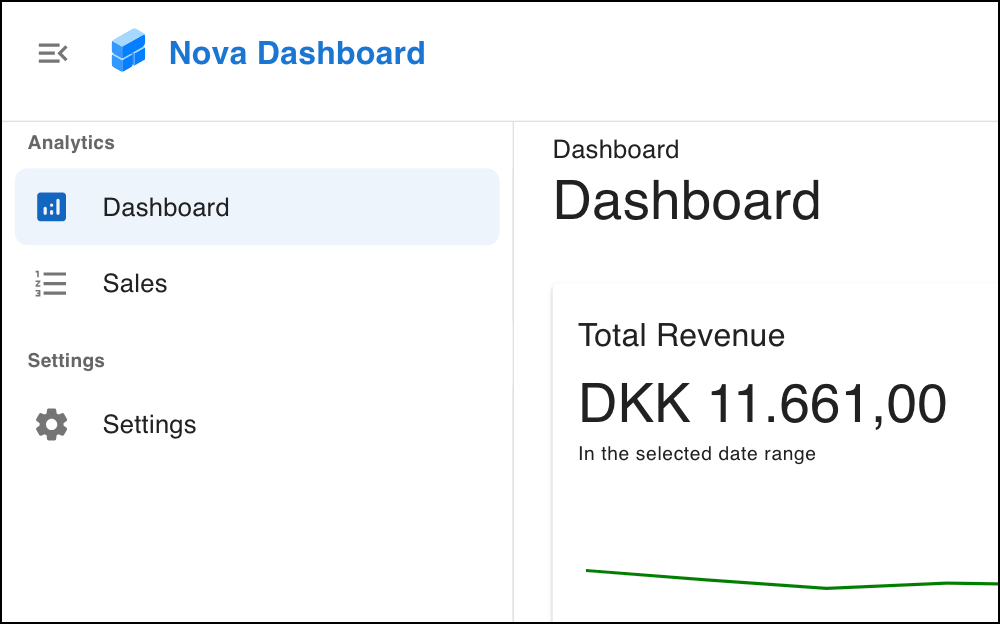
\includegraphics[width=.4\textwidth]{design-final-menu.png}
    \caption{Expanded hamburger menu.
    }\label{fig:design-final-menu}
\end{figure}

\subsection{Heuristics}\label{subsec:heuristics}

Throughout the design period, the group has kept a strong focus on Jakob Nielsen's 10 usability
heuristics~\cite{usability-heuristics}.
These are a set of general principles that can be used to evaluate the usability of a user interface.
While the group could not satisfy all the heuristics, many of them were taken into consideration when designing the
user interface.
The following is a list of the most relevant heuristics and how they were implemented in the design.

% textidote: ignore begin
\subsubsection{Visibility of system status}\label{subsubsec:visibility-of-system-status}
% textidote: ignore end

This heuristic is about keeping the user informed about what is happening.
It is achieved by showing a spinning wheel when the data is being loaded, and by showing a status notification
when order data is being imported or when settings are being saved.

% textidote: ignore begin
\subsubsection{Consistency and standards}\label{subsubsec:consistency-and-standards}
% textidote: ignore end

This heuristic is about making sure that the design is consistent.
By using the MUI library, explained in Section~\ref{subsec:front-end-libraries}, the group ensures that the design is
consistent.
Consistency is also achieved by using the same color scheme throughout the design.
The navigation bar and the filter options are also consistent across the different pages that support them.

% textidote: ignore begin
\subsubsection{Error prevention}\label{subsubsec:error-prevention}
% textidote: ignore end

This heuristic is about making sure that the user does not make mistakes.
The system has a number of error preventions, such as checks to make sure that the user is uploading the correct file.

% textidote: ignore begin
\subsubsection{Flexibility and efficiency of use}\label{subsubsec:flexibility-and-efficiency-of-use}
% textidote: ignore end

This heuristic is about making sure that the system can be used efficiently.
It is achieved by making the charts interactive and by allowing the user to filter the data.
Furthermore, the user can create categories for the charts, which allows for a more detailed analysis of the data.

% textidote: ignore begin
\subsubsection{Aesthetic and minimalist design}\label{subsubsec:aesthetic-and-minimalist-design}
% textidote: ignore end

This heuristic is about making sure that the design is aesthetically pleasing, by focusing on the content.
It is achieved by bringing the focus to the charts.
The libraries used for the interface and charts are also minimalistic in design, and the navigation bar is collapsible,
which creates more space for the charts.

